\documentclass{article}

% if you need to pass options to natbib, use, e.g.:
%     \PassOptionsToPackage{numbers, compress}{natbib}
% before loading neurips_2026
\PassOptionsToPackage{numbers, compress}{natbib}

% The authors should use one of these tracks.
% Before accepting by the NeurIPS conference, select one of the options below.
% 0. "default" for submission
% \usepackage{neurips_2026}
% the "default" option is equal to the "main" option, which is used for the Main Track with double-blind reviewing.
% 1. "main" option is used for the Main Track
%  \usepackage[main]{neurips_2026}
% 2. "position" option is used for the Position Paper Track
%  \usepackage[position]{neurips_2026}
% 3. "eandd" option is used for the Evaluations & Datasets Track
 % \usepackage[eandd]{neurips_2026}
 % if you want to opt-in for a de-anomymized submission (not recommended, but OK):
 %\usepackage[eandd, nonanonymous]{neurips_2026}
% 4. "creativeai" option is used for the Creative AI Track
%  \usepackage[creativeai]{neurips_2026}
% 5. "sglblindworkshop" option is used for the Workshop with single-blind reviewing
 % \usepackage[sglblindworkshop]{neurips_2026}
% 6. "dblblindworkshop" option is used for the Workshop with double-blind reviewing
%  \usepackage[dblblindworkshop]{neurips_2026}

% After being accepted, the authors should add "final" behind the track to compile a camera-ready version.
% 1. Main Track
 \usepackage[main, final]{neurips_2026}
% 2. Position Paper Track
%  \usepackage[position, final]{neurips_2026}
% 3. Evaluations & Datasets Track
 % \usepackage[eandd, final]{neurips_2026}
% 4. Creative AI Track
%  \usepackage[creativeai, final]{neurips_2026}
% 5. Workshop with single-blind reviewing
%  \usepackage[sglblindworkshop, final]{neurips_2026}
% 6. Workshop with double-blind reviewing
%  \usepackage[dblblindworkshop, final]{neurips_2026}
% Note. For the workshop paper template, both \title{} and \workshoptitle{} are required, with the former indicating the paper title shown in the title and the latter indicating the workshop title displayed in the footnote.
% For workshops (5., 6.), the authors should add the name of the workshop, "\workshoptitle" command is used to set the workshop title.
% \workshoptitle{WORKSHOP TITLE}

% "preprint" option is used for arXiv or other preprint submissions
 % \usepackage[preprint]{neurips_2026}

% to avoid loading the natbib package, add option nonatbib:
%    \usepackage[nonatbib]{neurips_2026}

\usepackage[utf8]{inputenc} % allow utf-8 input
\usepackage[T1]{fontenc}    % use 8-bit T1 fonts
\usepackage{hyperref}       % hyperlinks
\usepackage{url}            % simple URL typesetting
\usepackage{booktabs}       % professional-quality tables
\usepackage{amsfonts}       % blackboard math symbols
\usepackage{nicefrac}       % compact symbols for 1/2, etc.
\usepackage{microtype}      % microtypography
\usepackage{xcolor}         % colors
\usepackage{verbatim}
\usepackage{graphicx}
\usepackage{subcaption}
\usepackage{tikz}
\usetikzlibrary{shapes.geometric, arrows.meta, positioning, fit, backgrounds, calc}


% --- todo notes ---
% Comment out the next line (or pass [disable]) before camera-ready
% to suppress every \todo / \et / \as marker in one go.
\usepackage[colorinlistoftodos,prependcaption,textsize=small]{todonotes}
% \usepackage[disable]{todonotes}

% Per-author inline todo macros. Usage: \et{rephrase this} or \as{cite?}.
\newcommand{\et}[1]{\todo[inline,color=blue!20,size=\small]{\textbf{ET:} #1}}
\newcommand{\as}[1]{\todo[inline,color=green!20,size=\small]{\textbf{AS:} #1}}
% Margin variants (shorter notes that don't break the paragraph).
\newcommand{\etm}[1]{\todo[color=blue!20,size=\scriptsize]{ET: #1}}
\newcommand{\asm}[1]{\todo[color=green!20,size=\scriptsize]{AS: #1}}

% Note. For the workshop paper template, both \title{} and \workshoptitle{} are required, with the former indicating the paper title shown in the title and the latter indicating the workshop title displayed in the footnote. 
\title{Reward Hacking: Unit Tests vs Formal Specifications}


% The \author macro works with any number of authors. There are two commands
% used to separate the names and addresses of multiple authors: \And and \AND.
%
% Using \And between authors leaves it to LaTeX to determine where to break the
% lines. Using \AND forces a line break at that point. So, if LaTeX puts 3 of 4
% authors names on the first line, and the last on the second line, try using
% \AND instead of \And before the third author name.


\author{%
  Amar Shah\\
%   \thanks{Use footnote for providing further information
%     about author (webpage, alternative address)---\emph{not} for acknowledging
%     funding agencies.} \\
  \texttt{amarshah@cmu.edu} \\
  % examples of more authors
  \And
  Elanor Tang \\
  % Affiliation \\
  % Address \\
  \texttt{elanor@cmu.edu} \\
  % \AND
  % Coauthor \\
  % Affiliation \\
  % Address \\
  % \texttt{email} \\
  % \And
  % Coauthor \\
  % Affiliation \\
  % Address \\
  % \texttt{email} \\
  % \And
  % Coauthor \\
  % Affiliation \\
  % Address \\
  % \texttt{email} \\
}


\begin{document}


\maketitle


\section{Introduction}
\label{intro}

Reward hacking is a fundamental challenge in reinforcement learning (RL) where
an agent exploits loopholes in the reward function to achieve high rewards
without performing the intended task~\cite{rewardhacking}. This phenomenon can
lead to unintended consequences and suboptimal performance, posing a significant
threat to the safet and reliability of AI systems~\cite{anthropicrh}. As the
state of the art AI models continue to be post-trained in RL enovironements, the
risk of reward hacking becomes increasingly pertinent. 


In this work, we examine the propensity of reward hacking in programming tasks. We observe that when provided test cases, models will reward hack (eg. hardcode the test cases) 20\% of the time. We propose a 
potential solution: formal specifications~\cite{Verus}. Formal specfications provide a mathematical guarantee that a program obeys a specification for all available inputs. If a program satisfies a 
correct formal specification, it is guaranteed to be correct for all inputs, and thus reward hacking is not possible. While in practice,
formal specifications are difficult to write and underspecifications are
theoretically reward hackable. However, we empirically observe that formal 
specifications were rewawrd hacked 0\% of the time.

While this paints a rosy picture, there are still major challenges with formal verification. Formal languages are more difficult for LLMs to generate and places an additional burden: they must write a proof that their code satisfies the specification. This shows up in our results: LLMs are able to generate correct implementations for 70\% of the benchmarks when given test cases, but only 21\% when given formal specifications. Thus, while formal specifications may be a promising solution to reward hacking, there are still significant challenges to overcome before they can be widely adopted.



Our contributions are as follows:
\begin{itemize}
\item We propose formal specifications as a potential solution to reward hacking in programming tasks.
\item We develop a measure of reward hacking in programming tasks and use it to empirically evaluate the prevalence of reward hacking when using test cases versus formal specifications.
\item We find that reward hacking occurs 20\% of the time with test cases and 0\% of the time with formal specifications and discuss future work to address the challenges of using formal specifications in practice.
\end{itemize}

\subsection{Background}
\label{background}

A \emph{formal specification} mathematically describes the expected properties of a program. 
Unlike testing, which checks a finite set of inputs, 
formal specifications can quantify over all possible inputs, 
enabling them to provide guarantees over all possible program behaviors.
\emph{Formal verification} is the process of mathematically proving that a program satisfies its specification.
Thus, it shifts the burden from ensuring correctness of an entire implementation 
(which may have complex performance optimizations)
to ensuring correctness of a higher-level mathematical specification, 
an easier task. 

% typically using a verification tool to ensure proof correctness.

One state-of-the-art verification tool is Verus~\cite{Verus}, a semi-automated Rust verifier which 
has already been used at the intersection
of AI and verification \cite{AutoVerus,alphaverus,verussage,RAGVerus,vericode}. 
In Verus, users can write three kinds of code: 
\begin{itemize}
    \item \emph{spec} code describes higher-level program properties such as function pre- and post-conditions
    or loop invariants.
    \item \emph{proof} annotations help give Verus hints for proving an implementation satisfies its spec:
    Verus is semi-automated, meaning it can automatically prove many specifications, 
    but when more complex reasoning is required,
    it may need some help in knowing intermediate proof goals 
    or useful lemma calls.
    \item \emph{exec} code is simply regular Rust executable code. 
    During compilation, Verus erases spec and proof code, 
    leaving only the exec code: 
    there is no runtime performance cost associated with adding Verus proofs.
\end{itemize}
Verus is designed to integrate directly into Rust code: 
it relies on the Rust type-checker and uses Rust macros and annotations.
However, using Verus does involve some Verus-specific syntax, 
such as additional mathematical keywords or naming function outputs to describe their expected properties.

% Verus will then check if the code satisfies these requirements. 
% Note that Verus's verification result is only as good as the specification quality: 
% if the specification is incorrect or fails to capture all possible cases, 
% implementations verified against such specifications will also lack full guarantees.
% And since Verus specifications are checkable and compositional, they can serve as unambiguous descriptions of program intent---beyond what unit tests can capture. 
% Verus~\cite{Verus} has already been used in projects at the intersection
% of AI and verification \cite{AutoVerus,alphaverus,verussage,RAGVerus,vericode}. 

\section{Experimental Setup}
\label{results}

\subsection{Verification Tool}

We use Verus~\cite{Verus}, a semi-automated Rust verification tool with multiple prior applications at the intersection
of AI and verification \cite{AutoVerus,alphaverus,verussage,RAGVerus,vericode}. 

In Verus, users can write three kinds of code: 
\begin{itemize}
    \item \texttt{spec} code describes higher-level program properties such as function pre- and post-conditions
    or loop invariants.
    \item \texttt{proof} annotations give Verus hints for verifying proof goals:
    Verus is semi-automated, meaning it automatically proves many specifications, 
    but more complex proofs may require some help to determine intermediate proof goals 
    or useful lemma calls.
    \item \texttt{exec} code is Rust executable code. 
    During compilation, Verus erases spec and proof code, 
    leaving only the exec code: 
    thus, adding Verus proofs incurs no runtime performance cost.
\end{itemize}
Verus is designed to integrate directly into Rust code: 
it relies on the Rust type checker and uses Rust macros and annotations.
However, using Verus does involve some Verus-specific syntax, 
such as additional mathematical keywords or named function outputs to describe their expected properties.

\subsection{Experimental Design}
We limit this project's scope to reward hacking with few-shot prompts,
since this provides a preliminary comparison; 
we believe future RL training will amplify the results shown below.

\begin{enumerate}
    \item Our benchmark contains coding problems 
    with NL descriptions and formal Verus specs;
    we consider the formal Verus specs to be the ``gold-standard''
    ultimately defining the problems.
    \item We provide a model with only the NL descriptions, 
    and ask it to generate 
    (A) unit tests for evaluating this coding task and 
    (B) a formal Verus specification. 
    This generated spec may differ from the original gold-standard spec.
    \item For both (A) and (B), we check if the code produced also satisfies
    the gold-standard spec. 
    If it does not (and satisfies the unit tests/generated Verus spec), 
    we interpret this to mean the model successfully ``hacked''
    the reward mechanism. 
    We hypothesize we will see more reward hacking with unit tests,
    compared to the Verus generated specs.
\end{enumerate}
\begin{figure}[h]
\centering
\tikzset{
  box/.style={rectangle, rounded corners=3pt, draw, align=center,
              minimum width=2.0cm, minimum height=0.65cm, font=\small},
  goldbox/.style={box, fill=yellow!50, draw=orange!90!black, very thick},
  genbox/.style={box, fill=blue!30, draw=blue!80!black, very thick},
  rlbox/.style={box, fill=green!20, draw=green!60!black, very thick},
  evalbox/.style={box, fill=red!30, draw=red!80!black, very thick},
  arr/.style={-{Stealth[length=4pt]}, thick},
}
\begin{tikzpicture}[node distance=0.3cm and 1.0cm]

  % Top: benchmark input
  \node[goldbox, minimum width=3.4cm] (bench)
    {Benchmark\\{\footnotesize NL spec + gold Verus spec}};

  % NL spec fed to generator
  \node[rlbox, below=0.45cm of bench] (gen)
    {LLM Generator};
  \draw[arr] (bench) -- node[right, font=\footnotesize]{NL spec} (gen);

  % Two branches
  \node[genbox, below left=-.3cm and 1.2cm of gen]  (tests)
    {(A) Unit Tests};
  \node[genbox, below right=-.3cm and 1.2cm of gen] (spec)
    {(B) Generated Verus Spec};
  \draw[arr] (gen) -- (tests);
  \draw[arr] (gen) -- (spec);

  % RL training nodes
  \node[rlbox, below=0.35cm of tests] (rlA)
    {LLM Implementor\\{\footnotesize goal: pass unit tests}};
  \node[rlbox, below=0.35cm of spec]  (rlB)
    {LLM Implementor\\{\footnotesize goal: satisfy Verus spec}};
  \draw[arr] (tests) -- (rlA);
  \draw[arr] (spec)  -- (rlB);

  % Code outputs
  \node[box, below=0.35cm of rlA] (codeA) {Code A};
  \node[box, below=0.35cm of rlB] (codeB) {Code B};
  \draw[arr] (rlA) -- (codeA);
  \draw[arr] (rlB) -- (codeB);

  % Evaluation node
  \node[evalbox, minimum width=3.4cm,
        below=0.6cm of $(codeA)!0.5!(codeB)$] (eval)
    {Evaluate \\{\footnotesize reward hacking $\Leftrightarrow$ gold Verus spec not satisfied}};
  \draw[arr] (codeA) -- (eval);
  \draw[arr] (codeB) -- (eval);

  % Gold spec dashed arrow going around the right side
  \draw[arr, dashed, draw=orange!80!red!90!black, very thick] (bench.east)
        -- ++(4.2,0)
        |- (eval.east)
        node[pos=0.25, right, font=\small\bfseries, text=orange!80!red!90!black]{gold spec};

\end{tikzpicture}
\caption{Experimental setup. Both branches receive only the natural language specification as input. The dashed arrow indicates the gold-standard Verus specification used solely for final evaluation.}
\label{fig:setup}

\end{figure}

% Note: it's possible that the code produced by the models does satisfy the gold-standard specification,
%     but Verus rejects it due to insufficient proof annotations. 
%     If we find this to be the case, 
%     we would add a step between (3) and (4) which asks a model to add only proof annotations to the produced code,
%     to help Verus see that the implementation does satisfy the specification.

\textbf{Benchmark}: We use the HumanEval-Verus
dataset~\cite{alphaverus}, which has 78 coding tasks with
NL descriptions, formal Verus specs, and Rust
implementations satisfying the Verus specs. 
This is the largest known
benchmark with NL and formal Verus specs. 
We leave other benchmarks to future work.

\section{Results}\label{sec:results}

\paragraph{Setup.} We evaluated Qwen3-Coder on $70$ HumanEval-Verus
benchmarks~\cite{alphaverus}, each consisting of a natural-language description, a
gold-standard Verus specification, and a reference Rust implementation. For each
problem the model produced $5$ samples (pass@$5$) under each of the two reward
mechanisms described in Section~\ref{intro}: Branch A rewards passing
model-generated unit tests, Branch B rewards verification against a
model-generated Verus specification. Both branches were prompted with $5$
few-shot examples ($4$ correct implementations and $1$ deliberate reward hack,
included so the model is aware reward hacking is on the table). A sample is
labeled \emph{correct} only if it satisfies the gold-standard Verus
specification; this judgement is independent of the in-loop reward signal.

\paragraph{Headline numbers.}
Figure~\ref{fig:results-pass-at-k} summarizes the per-problem outcome
distribution for each branch.

\begin{figure}[h]
\centering
\begin{subfigure}[t]{0.48\textwidth}
  \centering
  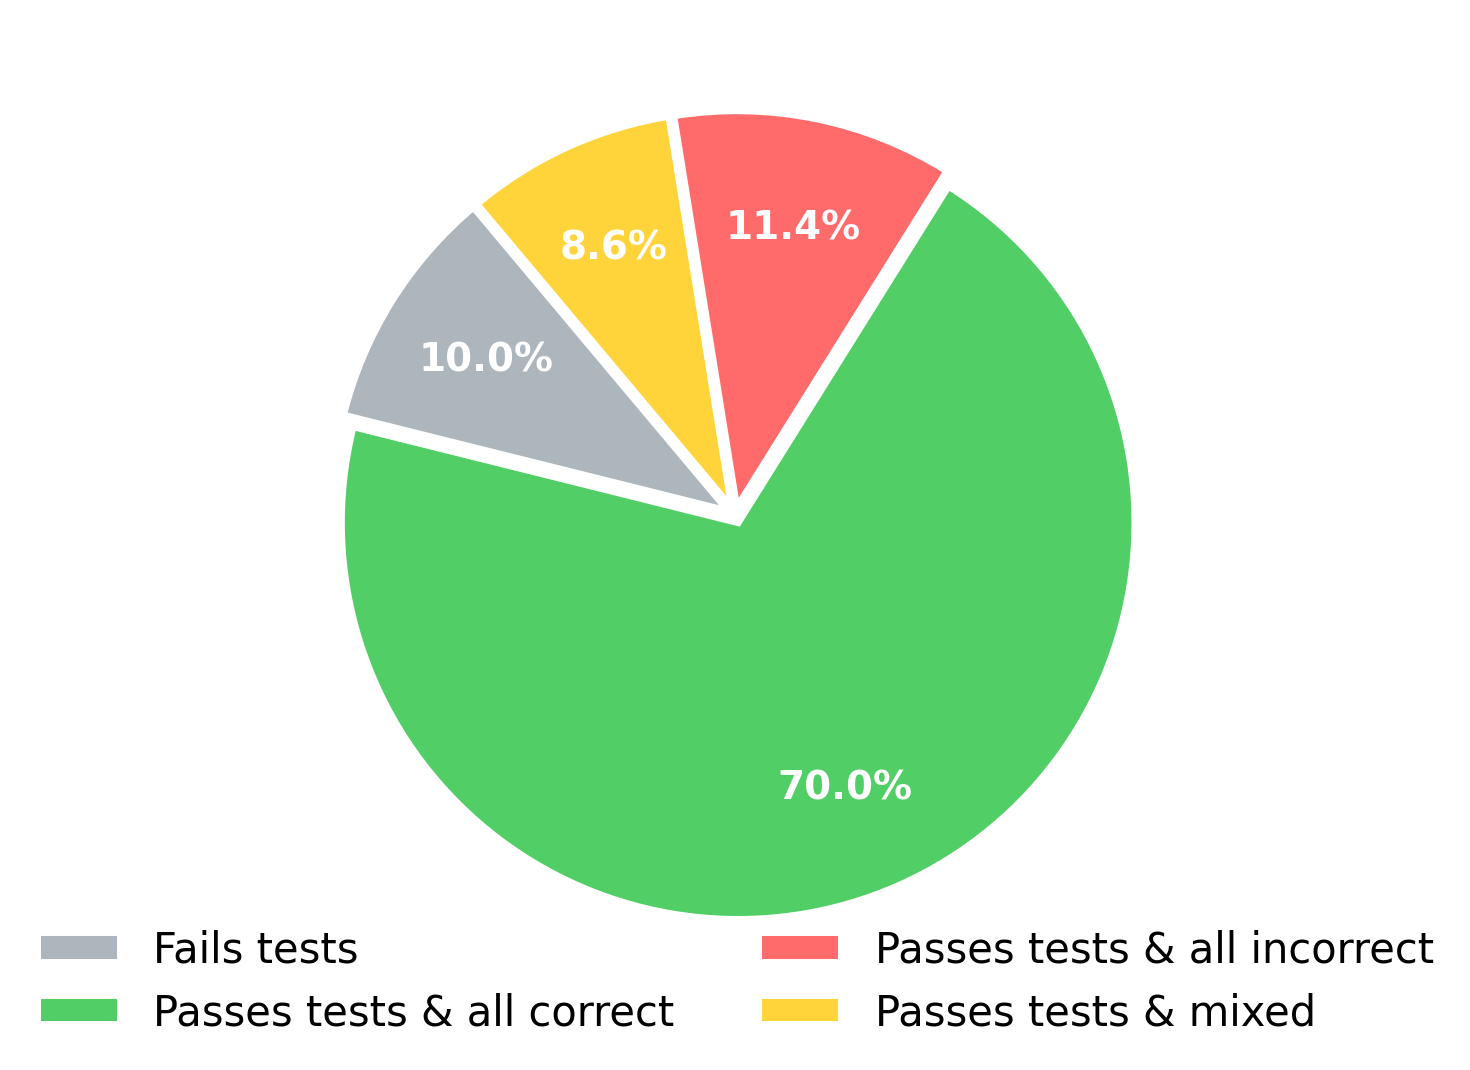
\includegraphics[width=\linewidth]{figures/branch_a2_pass_at_k.png}
  \caption{Unit-test reward (Branch A). Of 70 problems, $70.0\%$ pass the generated tests and are also judged correct against the gold-standard Verus specification. The remaining $20.0\%$ pass the tests despite being incorrect ($11.4\%$ all incorrect, $8.6\%$ a mix of correct and incorrect across the $5$ samples) -- these are reward hacks. The final $10.0\%$ fail the tests outright.}
  \label{fig:results:branch-a}
\end{subfigure}
\hfill
\begin{subfigure}[t]{0.48\textwidth}
  \centering
  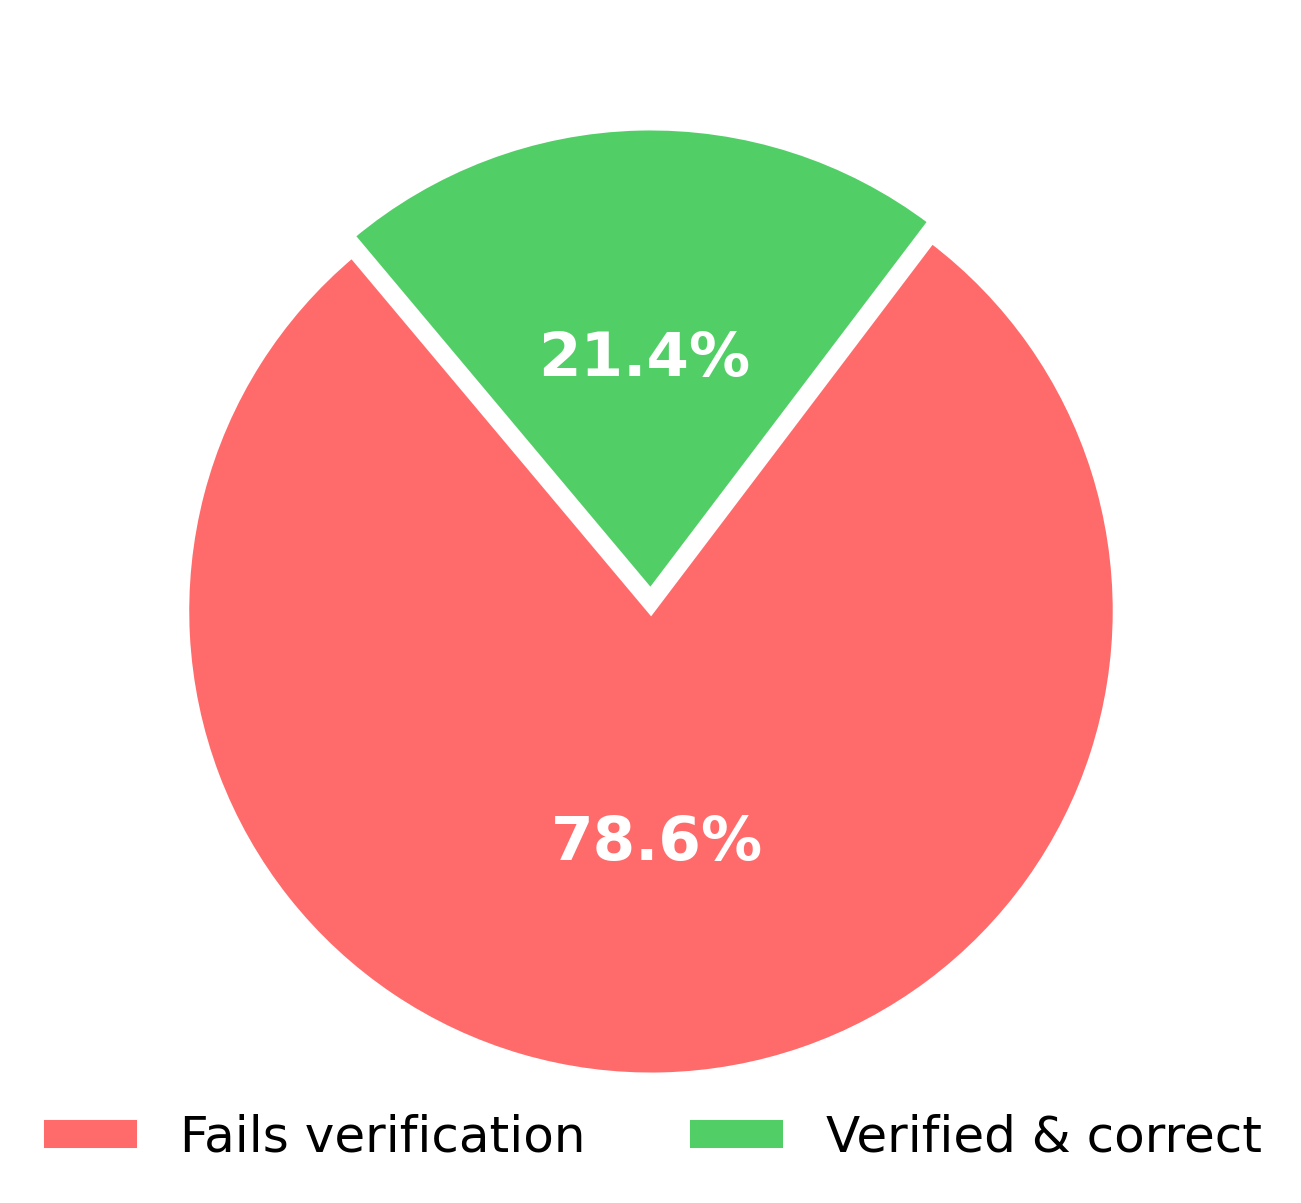
\includegraphics[width=\linewidth]{figures/branch_b_pass_at_k.png}
  \caption{Formal-spec reward (Branch B). Of 70 problems, $21.4\%$ are verified by Verus against the generated specification and judged correct against the gold-standard. The remaining $78.6\%$ fail verification. Crucially, $0\%$ of samples passed verification while being incorrect: with formal specifications, the model never reward-hacked.}
  \label{fig:results:branch-b}
\end{subfigure}
\caption{Outcome breakdown across $70$ HumanEval-Verus problems with Qwen3-Coder at pass@$5$. Reward hacking (passes the in-loop reward signal but is incorrect under the gold-standard spec) accounts for $20\%$ of unit-test outcomes (left) but $0\%$ of formal-spec outcomes (right).}
\label{fig:results-pass-at-k}

\end{figure}

Under the unit-test reward (Branch A), $70.0\%$ of problems are solved
correctly, but a further $20.0\%$ pass the generated tests while being incorrect
under the gold-standard specification ($11.4\%$ where every one of the $5$
samples is wrong, plus $8.6\%$ where the $5$ samples are a mix of correct and
incorrect implementations that all satisfy the tests). The remaining $10.0\%$
fail the tests outright. We interpret the $20.0\%$ slice as reward hacking:
the model produced code that the reward signal accepts but the
specification rejects. Manual inspection confirms the typical failure
mode is hard-coding the test inputs.

Under the formal-spec reward (Branch B), $21.4\%$ of problems are verified by
Verus and judged correct against the gold-standard, and the remaining $78.6\%$
fail verification. Notably, $0\%$ of samples passed verification while being
incorrect -- the model did not reward-hack. This is the property formal
specifications are supposed to give us: when the reward signal is a
machine-checked proof of a specification, hacking the reward requires producing
a verified-but-wrong program, which the soundness of Verus rules out (modulo
under-specification, which we did not observe in practice on these problems).

\paragraph{Takeaways.}
\begin{itemize}
\item \textbf{Reward hacking is empirically much rarer with formal specifications.}
  $20.0\%$ vs.\ $0\%$ on this benchmark.
\item \textbf{Reward hacking with formal specifications is not impossible in principle.}
  An under-specification that admits incorrect programs would still be reward
  hackable; we simply did not observe one here.
\item \textbf{Unit tests still produce more \emph{correct} code overall.} Branch
  A reaches $70.0\%$ true success vs.\ $21.4\%$ for Branch B. The bottleneck for
  Branch B is not specification quality but rather the model's ability to
  produce code together with proof annotations that Verus can check; we discuss
  this trade-off further in Section~\ref{challenges}.
\end{itemize}

\as{Experiments that we want to run next: varying model, A1 vs A2, increasing few-shot, pass@k}


\section{Challenges}
\label{challenges}

We encountered two significant challenges as we implemented our pipeline:
getting an LLM to generate correct Verus code, 
and checking if an implementation met the gold-standard Verus specification. 

\subsection{Generating Verus Code}

While LLMs are very familiar with Rust code, 
smaller LLMs have less experience with Verus-specific syntax.
Thus, they struggled to generate Verus code in multiple ways.
\begin{enumerate}
    \item The earliest failure mode was when
    the LLM generator failed to produce syntactically correct 
    Verus specifications from the NL description.
    \item The next case was during code generation for (B), 
    when the LLM implementation also failed to parse, 
    due to mistakes like using executable functions not supported by Verus,
    or incorrect proof/exec syntax.
    \item Even if the specification and implementation used correct syntax,
    the LLM could fail to generate the logically-correct proof annotations 
    needed to prove that the implementation satisfied the specification.
\end{enumerate}
We illustrate the failure breakdown in Figure [insert], 
which shows a more detailed analysis of Figure~\ref{fig:results-pass-at-k}(b).

We plan to address this challenge by providing more few-shot examples,
to help model correct Verus syntax,
and by giving more specific instructions in our prompt.

\subsection{Proving Correctness Against the Gold-Standard}

Our initial attempt was to give an LLM (Claude Opus [what version?]) 
the generated implementation and ask it to add only proof annotations, 
to help Verus see how the implementation satisfied the gold-standard specification;
if the LLM was unable to do so, we interpreted that to mean the implementation was incorrect.
However, even when strongly prompted against this, 
the LLM would occasionally modify the implementation to make it satisfy the specification.
Additionally, it is hard in general to verify an implementation which is written independently of the specification;
it was quite possible that the implementation was in fact correct, 
but the LLM was unable to determine the necessary proof annotations. 

Our next approach was to use the Verus gold-standard specifications to generate \emph{property-based tests}
which sample from the input space determined by the Rust type, 
subject to the constraints outlined in the specs.
Since we already had a gold-standard implementation which we know to be correct 
(since it satisfied the gold-standard specs), 
we could use that implementation to provide the expected correct output,
and test if the generated implementation gave the same output. 

However, it was difficult to achieve good coverage merely by sampling from the input space:
in many cases, the target function accepted all inputs of a given type,
but only did something interesting if that input took a specific form. 
Since sampling uniformly generated these inputs with very low probability,
we needed to add task-specific instructions to our test generation script.
This is not scalable.

We are currently exploring alternate approaches:
we want to try using an LLM to generate an input on which the generated implementation
and the gold-standard implementation differ, if it exists.
% Since having a concrete counter-example only guarantees that the implementations differ 
% (as the lack of a counter-example is not a guarantee that they are the same),
% we would do this in combination with a test suite.
We also want to try generating tests based on the gold-standard \emph{implementation} rather than the specification,
in a way that achieves full coverage over all control branches of the implementation.
We hope this would solve the issues of merely sampling over the input space.

\section{Future Work}
\label{futurework}

Once we address the challenges outlined in the previous section, 
we plan to run rejection fine-tuning on the code generation part of our pipeline, 
to see if this amplifies reward-hacking behavior.
We would use satisfying the unit tests/generated Verus specification as the reward
and train on traces which satisfy the reward but are not actually correct. 

More generally, we also want to see if we can somehow get the best of both worlds,
combining the ease of unit testing and the guarantees of formal specification. 
This would include further investigation into methods like fuzzing and property-based testing, 
as well as looking into ways that we can improve the shortfalls of using formal specs.



\begin{ack}
% TODO: write acknowledgements.
\end{ack}

\bibliographystyle{plain}
\bibliography{references}


%%%%%%%%%%%%%%%%%%%%%%%%%%%%%%%%%%%%%%%%%%%%%%%%%%%%%%%%%%%%

\appendix

%%%%%%%%%%%%%%%%%%%%%%%%%%%%%%%%%%%%%%%%%%%%%%%%%%%%%%%%%%%%


\end{document}